 	\documentclass[aspectratio=169]{beamer}

\usepackage[utf8]{inputenc}

\usepackage{graphicx}
\usepackage{caption}
\usepackage{subfigure}

\graphicspath{{pictures/}}
\DeclareGraphicsExtensions{.pdf,.png,.jpg}

\usepackage{amsmath,amsfonts,amssymb,amsthm,mathtools}
\usepackage[main=russian,english]{babel}
%\usepackage[T1]{fontenc}

\title{Скин--эффект}
\date{\small{МФТИ, Долгопрудный 2021}}
\author{\small{Крейнина Матвея \\ студент 2 курса группы Б05-005}}


\usetheme{texsx}
%\usetheme{gcr2019}

\begin{document}
%1	-	Первый слайд
\begin{frame}
  \frametitle{\textcolor{white}{Вопрос по выбору}} 
	\titlepage
\end{frame}
%2  - Введение
\begin{frame}
\frametitle{\textcolor{white}{Распределение токов}} 
Рассмотрим вопрос о распределении переменных токов по сечению проводников.
Этот вопрос важен не только с теоретической, но и с технической точки зрения. Даже в однородном квазилинейном проводнике переменный ток в отличие от постоянного не распределяется равномерно по сечению проводника, а концентрируется на его поверхности.

Это явление получило название скин-эффект. Т.е. ток концентрируется на <<коже>> проводника, что в свою очередь влечет за собой изменение эффективного сопротивления и самоиндукции проводника.


При выводе уравнения будем исходить из основных уравнений электромагнитного поля:
\begin{equation*}
rot E = - \frac{1}{c} \frac{\partial B}{\partial t} = - \frac{\mu}{c} \frac{\partial H}{\partial t}, rot H = \frac{4 \pi \lambda}{c}E + \frac{1}{c}\frac{\partial D}{\partial t}
\end{equation*}
\end{frame}

%3	- Вывод соотношений
\begin{frame}
\frametitle{\textcolor{white}{Вывод соотношений}}
Так как плотность токов смещения в проводниках, по крайне мере, в металлах мала по сравнению с плотностью токов проводимости, мы можем пренебречь вторым членом и положить. 

\begin{equation*}
	rotH = \frac{4 \pi \lambda}{c} E
\end{equation*}

Рассмотрим однородный проводник, на протяжении которого $\varepsilon, \lambda$ и $\nu$ величины постоянные. 

Получаем
\begin{equation*}
 rot (rot E) = - \frac{\mu}{c} \frac{\partial}{\partial t}(rot H) = -\frac{4 \pi \mu \lambda}{c^2}  \frac{\partial E}{\partial t}
\end{equation*}

С другой же стороны:
\begin{equation*}
rot(rot E) = grad(divE) - \nabla^2E
\end{equation*}
\end{frame}

%4	- Вывод соотношений
\begin{frame}
\frametitle{\textcolor{white}{Вывод соотношений}}
При этом, если внутри проводника нет объёмных зарядов, т.е. $\rho = 0$, из постоянства $\varepsilon$ будет следовать, что
\begin{equation*}
div D = div \varepsilon E = \varepsilon div E = 0
\end{equation*}

Получается, что уравнение принимает следующий вид:
\begin{equation*}
\nabla^2 E = \frac{4 \pi \mu \lambda}{c^2} \frac{\partial E}{\partial t}
\end{equation*}

Таким же образом можно и получить для магнитного вектора H:
\begin{equation*}
\nabla^2 H = \frac{4 \pi \mu \lambda}{c^2} \frac{\partial H}{\partial t}
\end{equation*}
\end{frame}

%5	- Вывод соотношений
\begin{frame}
\frametitle{\textcolor{white}{Вывод соотношений}}
Ограничимся рассмотрением переменных полей, напряженность которых является синусоидальной функцией времени, и будем выражать их напряженность в комплексной форме:

\begin{equation*}
E = E_0(x, y, z)e^{i \omega t}
H = H_0(x, y, z) e^{i \omega t}
\end{equation*}

Амплитуды $E_0$ и $H_0$ могут быть комплексными векторами, но от времени не будут зависеть.


Подставим $E = E_0(x, y, z)e^{i \omega t}$ в уравнение: $\nabla^2 E = \frac{4 \pi \mu \lambda}{c^2} \frac{\partial E}{\partial t}$ и сократим на $e^{i \omega t}$.

Получим:
\begin{equation*}
\nabla^2 E_0 = \frac{4 \pi \mu \lambda i \omega}{c^2} E_0 = 2ip^2E_0, \text{где } p^2 = 2 \pi \mu \lambda \omega/c^2
\end{equation*}
\end{frame}

%6	- Рассмотрение случая
\begin{frame}
\frametitle{\textcolor{white}{Простейший случай}}

Пусть у нас есть бесконечный однородный проводник, который занимает полупространство $z > 0$ таким образом, что его поверхность совпадает с плоскостью $z = 0$.

Предположим, что электрическое поле, а следовательно и ток направлены по оси x параллельно граничной поверхности ($E_y = E_z = 0$).
\begin{center}
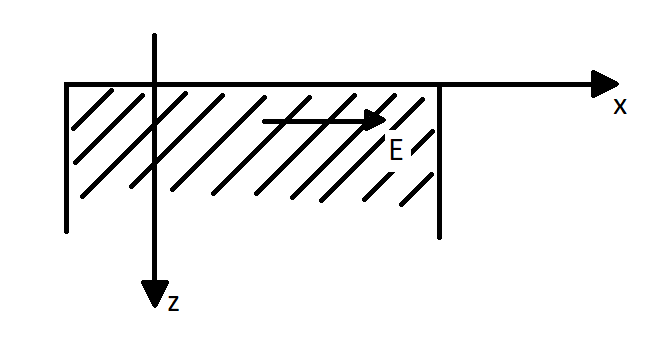
\includegraphics[scale=0.5]{01.png}
\end{center}
Следующим предположением будет то, что поле зависит только от расстояния z  рассматриваемой точки проводника от его поверхности, но не зависит от x и y.
\end{frame}

%7	- Простейший случай
\begin{frame}
\frametitle{\textcolor{white}{Простейший случай}}
Тогда уравнение принимает вид:
\begin{equation*}
\nabla^2 E_{0x} = \frac{\partial^2 E_{0x}}{\partial z^2} = 2ip^2E_{0x}
\end{equation*}

Общее решение такого уравнения, как известно, имеет вид:
\begin{equation*}
E_{0x} = Ae^{kz} + Be^{-kz}, \text{ где A и B - постоянные интегрирования}
\end{equation*}
k - корень уравнения: $k^2  =2ip^2$, т.е. $k = p \sqrt{2i} = p (1 + i)$

Таким образом:
\begin{equation*}
E_{0x} = Ae^{pz}e^{ipz} + Be^{-pz}e^{-ipz}
\end{equation*}
Так как величина p -- вещественная, то мы должны положить коэффициент A равным нулю, иначе при отдалении вглубь проводника поле $E_0$ росло бы до бесконечности.
\end{frame}

%8	- Простейший случай
\begin{frame}
\frametitle{\textcolor{white}{Простейший случай}}
Переходя от амплитуды электрического вектора к его полному комплексному выражению, получим:

\begin{equation*}
E_x = E_{0x}e^{i \omega t} = B e^{-pz}e^{i(\omega t - p z)}
\end{equation*}
Отбросив мнимую часть, получаем:
\begin{equation*}
E_x = Be^{-pz}cos(\omega t - pz)
\end{equation*}
Тогда для плотности тока получим:
\begin{equation*}
j_x = \lambda E_x = j_0 e^{-pz}cos(\omega t - pz), j_0 = \lambda B
\end{equation*}

Получаем, что по мере проникновения в глубь проводника фаза электрического вектора и плотности тока изменяются линейно, а амплитуды убывают по экспоненте. 
Основная часть тока сосредоточена в поверхностном слое толщиной в $1/p$ см, т.к. на этой глубине плотность тока уже в e раз меньше. 
\end{frame}

%9	- Оценка
\begin{frame}
\frametitle{\textcolor{white}{Оценка}}
Чтобы оценить толщину этого слоя, рассмотрим конкретный пример.
Для меди:

$\mu = 1, \lambda = 6 \cdot 10^{-4} $ эл.-маг. ед. $= c^2 \cdot 6 \cdot 10^{-4} $абс. (эл. стат.) ед.

Циклическая частота равна: 
\begin{equation*}
w = 2 \pi / T = 2 \pi \nu
\end{equation*}
При 1000 периодах получаем: 
\begin{equation*}
p = \sqrt{2 \pi \mu \lambda \omega / c^2} \sim 5 \text{  см}^{-1}
\end{equation*}
При $10^5$ периодах в секунду (медленные радиотелеграфные колебания, длина волны 3000 м), получаем:
\begin{equation*}
p \sim 50 \text{  см}^{-1}
\end{equation*}

Таким образом в первом случае ток сосредоточен в слое толщиной $1/5 \text{  см} = 2 \text{  мм}$, а во втором -- в слое всего лишь $1/50 \text{  см} = 0.2 \text{  мм}$.
При $\omega = 0$,	 $p = 0$  напряженность поля и сила тока сохраняют постоянное значение по всей толщине проводника.
\end{frame}

%10	- Выводы
\begin{frame}
\frametitle{\textcolor{white}{Выводы}}
Результаты, полученные при рассмотрении бесконечного проводника качественно, применимы к наиболее интересному случаю цилиндрических проводников. И в этом случае переменный ток концентрируется на поверхности проводника тем сильнее, чем больше частота тока. Концентрация тока на поверхности влечет за собой изменение сопротивления и самоиндукции проводника. Таким образом, для переменных токов эти величины уже не являются постоянными, а зависят от частоты тока. Например, если весь ток концентрируется на поверхностном слое цилиндрического провода, то сопротивление должно стать равным сопротивлению полого цилиндра, обладающего стенками соответствующей толщины. При увеличении частоты толщина проводящего ток слоя уменьшается, т.е. сопротивление проводника должно увеличаться.
\end{frame}

%11	- Альтернативный вывод
\begin{frame}
\frametitle{\textcolor{white}{Альтернативный вывод}}
\begin{center}
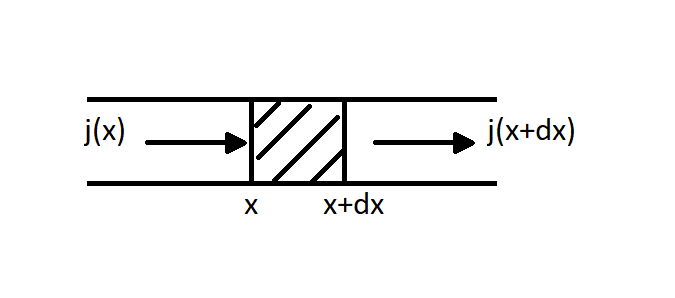
\includegraphics[scale=0.5]{02.png}
\end{center}

Если j(x) -- плотность диффузионного тока, то приращение в единицу времени числа частиц в слое, заштрихованном на рисунке, представится разностью:
$j(x) - j(x+dx) = -\frac{\partial j}{\partial x} dx$. Это же приращение равно: $\frac{\partial n}{\partial t} dx$

Получаем:
\begin{equation*}
\frac{\partial j}{\partial x} = - \dot n \text{  ,  }j = - D \frac{\partial n}{\partial t}
\end{equation*}
D -- коэффициент диффузии.
\end{frame}

%12	- Альтернативный вывод
\begin{frame}
\frametitle{\textcolor{white}{Альтернативный вывод}}
Выделим теперь в трубе столб вещества длинной l. Пусть в начальный момент времени на левом конце этого столба концентрация n отлична от нуля, а на правом обращается в нуль. Также допустим, что концентрация n равна нулю во всех точках трубы, расположенных правее выделенного столба. 

Плотность диффузионного тока: 
\begin{equation*}
j \sim Dn/l 
\end{equation*}
Ту же величину можем представить, как $j = nv$, где v -- скорость, с которой вещество при диффузии распространяется вдоль трубы.

Отсюда получаем: 
\begin{equation*}
v \sim D/l
\end{equation*}

Время $\tau$, за которое вещество диффундирует на расстоянии l, будет: $\tau \approx l/v \approx l^2/D$, следовательно:
\begin{equation*}
l \sim \sqrt{D \tau}
\end{equation*}
\end{frame}

%13	- Альтернативный вывод
\begin{frame}
\frametitle{\textcolor{white}{Альтернативный вывод}}

Теперь перейдем к задаче о проникновении электромагнитного поля в металл. Пренебрегая токами смещения, этот процесс будет описываться уравнениями:
\begin{equation*}
rot H = \frac{4 \pi}{c} j, rot E = - \frac{1}{c} \dot B
\end{equation*}
Используя соотношения: 
\begin{equation*}
j = \lambda E \text{и} B = \mu H,
\end{equation*}

исключим из этих уравнений E и H.

Получим:
\begin{equation*}
j = \frac{c}{4 \pi \mu} rot B, rot j = -\frac{\lambda}{c} \dot B
\end{equation*}

\end{frame}

%14	- Альтернативный вывод
\begin{frame}
\frametitle{\textcolor{white}{Альтернативный вывод}}
Допустим, что все величины зависят от одной координаты x, и для этого случая запишем полученные уравнения в координатной форме.
\begin{equation*}
\frac{\partial j}{\partial x} = - \frac{\lambda}{c} \dot B, j = - \frac{c^2}{4 \pi \mu \lambda} \frac{\partial}{\partial x} \left( \frac{\lambda}{c} B \right)
\end{equation*}
Произведем замену: 
\begin{equation*}
n \rightarrow (\lambda/c)B
\end{equation*}
и положим: 

\begin{equation*}
D = \frac{c^2}{4 \pi \mu \lambda}
\end{equation*}

Таким образом, распространение электромагнитного поля в металле описывается уравнениями диффузии, роль коэффициента диффузии играет величина D.

\end{frame}

%15	- Оценка проникновения
\begin{frame}
\frametitle{\textcolor{white}{Оценка}}
Допустим, теперь, что по плоской поверхности металла начинает течь переменный ток,  периодически меняющийся во времени с периодом T.
Через половину периода T/2 ток изменит направление на противоположное. За это время электрическое поле, а с ним и электрический ток успеют проникнуть внутрь на глубину:
\begin{equation*}
l \sim \sqrt{D \frac{T}{2}} \sim c \sqrt{\frac{T}{8 \pi \mu \lambda}} \sim \frac{c}{\sqrt{8 \pi \mu \lambda \nu}}
\end{equation*}
Сравним с ранее полученным результатом:
\begin{equation*}
p^{-1} =  \frac{c}{\sqrt{2 \pi \mu \lambda \omega}}
\end{equation*}

Видно, что оценка с диффузией тока с точностью до коэффициента совпадает с точно полученными результатами.
\end{frame}




%16	- Выводы
\begin{frame}
\frametitle{\textcolor{white}{Вывод}}
В отличие от сопротивления, самоиндукция проводника уменьшается по мере увеличения частоты тока. Самоиндукция проводника, согласно определению, пропорциональна энергии магнитного поля тока, циркулирующего по этому проводнику. С другой стороны, известно, что если ток сосредоточен на поверхности цилиндрического проводника, то магнитное поле внутри проводника равно нулю. Поле же вне цилиндра от распределения тока по его сечению не зависит. Следовательно, по мере концентрации тока на поверхности проводника уменьшается энергия его поля, а стало быть, и самоиндукция проводника, причем последняя стремится к пределу L', равному внешней самоиндукции проводника.
\end{frame}

\end{document}